\section{Description de la structure}\label{sec:DescStruct}
Avant de commencer à regarder les différentes solutions des points clés du projet il convient de se mettre d'acoord
sur la structure principale où tout sera attaché. Cette dernière est faîte en profilé Item \cite{Item} comme convenu dans le decriptif
du projet. Afin de pouvoir le placer sur une table comme demandé, l'installation de pieds sera nécessaire. Les pieds proposé par Item ne
permettent pas une adhérence suffisante à la table et ne sont pas réglables. Elesa \cite{Elesa} possède une grande variété de pieds ce qui
a permis de trouver exactement ce qui était recherché pour ce projet. La fabrication d'une pièce (plan dans les Annexes) pour pouvoir attacher
les pieds au reste de la structure est donc nécessaire.

\begin{figure}[H]
    \centering
    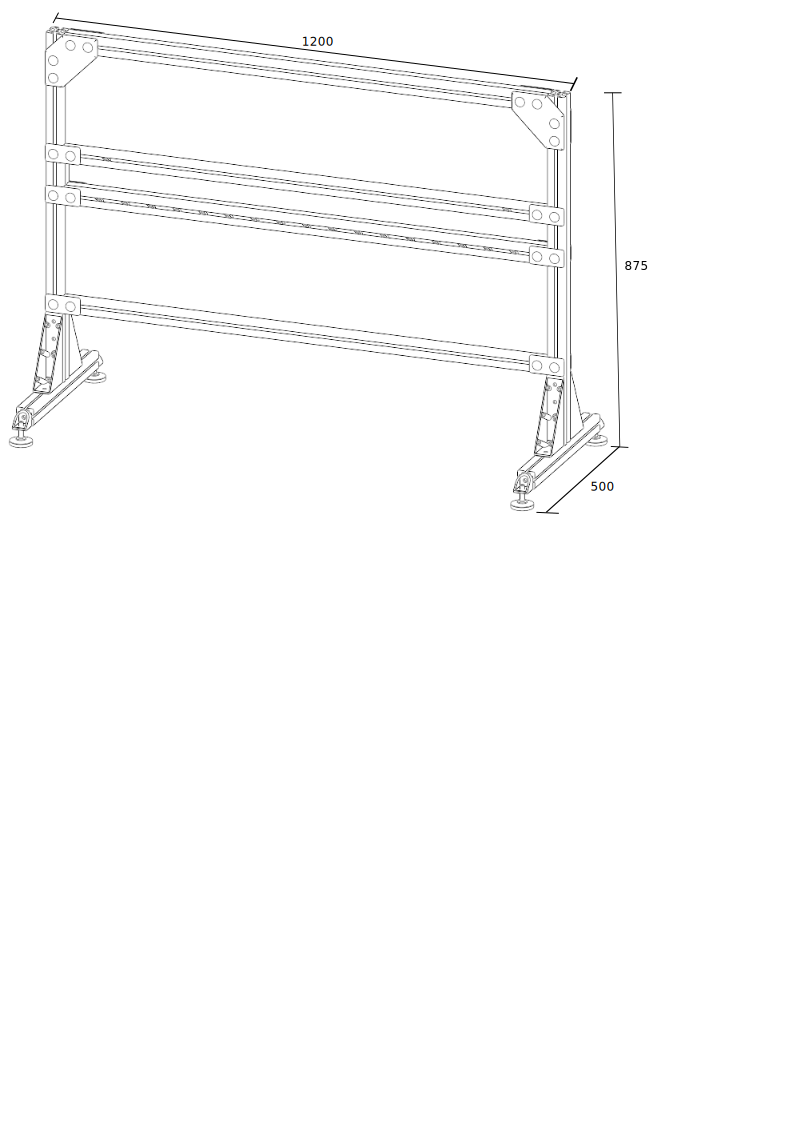
\includegraphics[width = 0.8\textwidth]{assets/figures/Structure.png}
    \caption{Représentation de la structure en 3D}
    \label{fig:DescStruct}
\end{figure}

On peut voir que la structure utilise quatre grands profilés horizontaux, deux aux extrémités et deux au centre. Ce sera sur les deux profilés du centre que
les éléments du pendule pourront venir se fixer plus tard. Deux plaques sont mises entre des profilés pour à la fois rendre le projet présentable
en cachant les éléments arrière et à la fois rendre la structure plus rigide.

\section{Catalogue de solutions}\label{sec:CatSol}
Maintenant que la structure est connue, il est possible d'étudier les différentes solutions sur les points clés du projet.
Les points principaux sont: le moteur linéaire, le guidage et la mesure de position linéaire.

\subsection{Moteur linéaire}
\subsubsection{A: Commander un moteur linéaire}
Les offres suivantes ont été faites par des entreprises contactées lors de ce travail.

\begin{table}[H]
    \centering
    \caption{Offres pour le moteur linéaire}
    \label{tab:OffreMot}
    \resizebox{\textwidth}{!}{%
        \begin{tabular}{|l|l|l|l|l|}
            \hline
            Entreprise               & Prix                       & Délai de livraison              & Poids chariot          & Force continue \\ \hline
            DD auto Tech             & 1105 CHF                   & \cellcolor{red}16 semaines      & 60g                    & 39N            \\ \hline
            ESR Pollmeier            & -                          & \cellcolor{red}16 semaines      & \cellcolor{yellow}600g & 29N            \\ \hline
            TDS Precision   Products & 1020 CHF                   & \cellcolor{yellow}8-10 semaines & 180g                   & 26.4N          \\ \hline
            Heidenhain/Etel          & \cellcolor{yellow}3000 CHF & 7 semaines                      & 100g                   & 31.9N          \\ \hline
        \end{tabular}%
    }
\end{table}

L'offre la plus intéressante est celle de TDS Precision avec un prix raisonnable et un temps de livraison un peu plus long mais qui rentre dans le planning.

\subsubsection{B: Utiliser un rail magnétique déjà en stock}
Un rail magnétique Etel de 1024mm de longueur est en stock à la HEIG et nécessiterait uniquement la commande de la partie mobile. Cependant ce
rail est plus lourd et encombrant que certaines des solutions commandables. Cela reste un bon plan de secours en cas de problème d'approvisionement.

\subsection{Guidage linéaire}
\subsubsection{A: Commander un guidage linéaire avec mesure de position intégré}
Les offres suivantes ont été faites par des entreprises contactées lors de ce travail.

\begin{table}[H]
    \centering
    \caption{Offres pour le guidage linéaire avec mesure de position}
    \label{tab:OffreGuidPos}
    \resizebox{\textwidth}{!}{%
        \begin{tabular}{|l|l|l|l|l|}
            \hline
            Entreprise   & Prix                             & Délai de livraison & Longueur & Poids chariot                \\ \hline
            Schneeberger & \cellcolor[HTML]{FF0000}1369 CHF & 4 semaines         & 995mm    & 84g                          \\ \hline
            Hiwin        & \cellcolor[HTML]{FF0000}1171 CHF & 3 semaines         & 1100mm   & \cellcolor[HTML]{FF0000}420g \\ \hline
        \end{tabular}%
    }
\end{table}

L'offre la plus intéressante est celle de Schneeberger avec un chariot beaucoup plus léger, cependant le prix est trop élevé pour pouvoir considérer cette solution.

\subsubsection{B: Commander guidage linéaire et le capteur de position séparément}
\textbf{ - Capteur:}
\newline
Les offres suivantes ont été faites par des entreprises contactées lors de ce travail.

\begin{table}[H]
    \centering
    \caption{Offres pour le capteur pour la mesure de position}
    \label{tab:OffrePos}
    \resizebox{\textwidth}{!}{%
        \begin{tabular}{|l|l|l|l|l|}
            \hline
            Entreprise & Prix                             & Délai de livraison                  & Longueur                       & Poids tête                  \\ \hline
            RLS        & \cellcolor[HTML]{FFFFFF}640 CHF  & \cellcolor[HTML]{FFFFFF}4 semaines  & \cellcolor[HTML]{FFFFFF}1000mm & 32g                         \\ \hline
            Heidenhain & \cellcolor[HTML]{FFFF00}1080 CHF & \cellcolor[HTML]{FF0000}16 semaines & \cellcolor[HTML]{FFFFFF}1040mm & \cellcolor[HTML]{FFFFFF}20g \\ \hline
        \end{tabular}%
    }
\end{table}

\textbf{ - Guidage:}
\newline
Les offres suivantes ont été faites par des entreprises contactées lors de ce travail.

\begin{table}[H]
    \centering
    \caption{Offres pour le guidage}
    \label{tab:OffreGuid}
    \resizebox{\textwidth}{!}{%
        \begin{tabular}{|l|l|l|l|l|}
            \hline
            Entreprise & Prix    & Délai de livraison & Longueur & Poids chariot                \\ \hline
            Ewellix    & -       & -                  & 995mm    & \cellcolor[HTML]{FF0000}400g \\ \hline
            Rollon     & -       & -                  & 1000mm   & 170g                         \\ \hline
            Igus       & 130 CHF & 10 jours           & 1100mm   & \cellcolor[HTML]{FFFF00}260g \\ \hline
            Igus       & 150 CHF & 2 jours            & 1100mm   & \cellcolor[HTML]{FFFFFF}110g \\ \hline
        \end{tabular}%
    }
\end{table}

Les deux offres choisies sont donc la règle linéaire de RLS et le second rail linéaire de Igus. Le poids minime du chariot Igus est un avantage considérable
et le temps de livraison plus court chez RLS sont les facteurs clés de ce choix.

\subsubsection{C: Commander guidage linéaire et utiliser un capteur déjà en stock}
\textbf{ - Capteur:}
\newline
Le capteur en stock est une règle linéaire LIDA 405 de 840mm de plage mesurable avec la tête de lecture et fixation. La seule partie à commander
est le support pour le ruban. Cette solution nécessite un temps de livraison inférieur à ceux des capteurs commandables et coute beaucoup moins cher.

\textbf{ - Guidage:}
\newline

\begin{table}[H]
    \centering
    \caption{Offres pour le guidage}
    \label{tab:OffreGuid}
    \resizebox{\textwidth}{!}{%
        \begin{tabular}{|l|l|l|l|l|}
            \hline
            Entreprise & Prix    & Délai de livraison & Longueur & Poids chariot                \\ \hline
            Ewellix    & -       & -                  & 995mm    & \cellcolor[HTML]{FF0000}400g \\ \hline
            Rollon     & -       & -                  & 1000mm   & 170g                         \\ \hline
            Igus       & 130 CHF & 10 jours           & 1100mm   & \cellcolor[HTML]{FFFF00}260g \\ \hline
            Igus       & 150 CHF & 2 jours            & 1100mm   & \cellcolor[HTML]{FFFFFF}110g \\ \hline
        \end{tabular}%
    }
\end{table}

Cette solution utilisera la règle linéaire de chez Heidenhain en stock et le second rail Igus grâce au poids minime de son chariot.

\section{Solutions choisies}\label{sec:SolChoix}

La solution choisie pour le moteur linéaire est la solution A, c'est à dire la commande d'un nouveau moteur chez TDS Precision. Ce dernier
sera fixé à l'arrière de la structure sur un des profilé du centre.\\

La solution choisie pour le guidage linéaire est la solution C, c'est à dire la commande d'un guidage linéaire chez Igus et l'utilisation d'une
règle linéaire de chez Heidenhain appartenant déjà à la HEIG. Le rail peut être fixé sur la partie avant des profilés et la règle linéaire peut
être placée sur la partie arrière du deuxième profilé.